\section{Implementation}
\ninanotes{
\begin{itemize}
\item Implementation
\item Describe how the design is turned into a program.
\item Describe how the design components are turned into software
components.
\item Mention the methods/algorithms you use, if necessary describe them.
\item Visualize the program structure if possible.
\item Do not list standard code, but specifically smart coding.
\end{itemize}
}


\subsection{Going through all permutations}
In sections \ref{sec:how-should-an-agent-play} and \ref{sec:design:removing-worlds-based-on-hints}, a key thing that has to be done in order to evaluate whether a hand with unknown cards but with some hints is part of a possible world, and defining each cards actionable states is through checking the permutations of a possible world.
Generating permutations can be done using Heap's algorithm \cite{wiki:heapsalgorithm}, which seem to be fast and not need that much data in order to compute the permutations. If there are $k$ objects, you only need to store $O(k)$ elements. My implementation is in "{\tt src/multi\_agent\_solvers/PermutationIterator.zig}". 

\subsection{Representing the world}
I mentioned that I picked the table representation from the different choices I had (see section \ref{sec:representing-a-world}), but I was not aware, at the time, of how byte-addressability would affect the actual space, so I was surprised that the space was filled up so quickly. There are ways to mitigate these problems of space by using porting the current encoding of 25 bytes, to make a packed array that uses bitmanipulation in order to achieve this \footnote{Zig has this in its library \cite{packed_int_array}}. Due to time constraints I chose to have only 1 agent with 1 model at a time, so that the agents in total do not use too much memory.

\subsection{Implementing the board game}
I also implemented the board game, simply referred to as the Game struct (in file "{\tt src/hanabi\_board\_game.zig}) in order for the agents to interact with the game. The board game keeps track on who is the current player and has some simple methods that the agents can use when they want to make a move:

\begin{itemize}
	\item {\tt play(index)}
	\item {\tt discard(index)}
	\item {\tt hint\_color(color, index\_of\_player) }
	\item {\tt hint\_value(value, index\_of\_player) }
\end{itemize}
In order to simplify the implementation of the board game, I simply let it crash if a agent does something that is illegal. (Like giving an index that is out of bounds, or hinting a color not on the hinted players hand).


\subsection{Agents}
The logical agents in the game are implemented as an Agent struct. See a class diagram on Figure \ref{fig:Agent-class-diagram}.
An Agent has a hand that is represented with {\tt CardWithStates}, here the states refer to each cards actionability (related to section \ref{sec:how-should-an-agent-play}), but also its hints. It does not see the actual cards. It has a {\tt KripkeStructure} which is its epistemic model. And lastly it has a {\tt CurrentPlayerView} which is the current game that the agent as a player is able to see i.e. it cannot see its own hand, or the contents of the deck. An Agent has a method called {\tt init(...)}, that based on the view and which player it is, is able to generate the entire model, as well as decide what states the {\tt CardWithStates} should be in. After an Agent has been {\tt init}ed it can make a move with the method {\tt make\_move(game)}, which modifies the game based on its {\tt hand}, as well as its view.

\begin{sidewaysfigure}
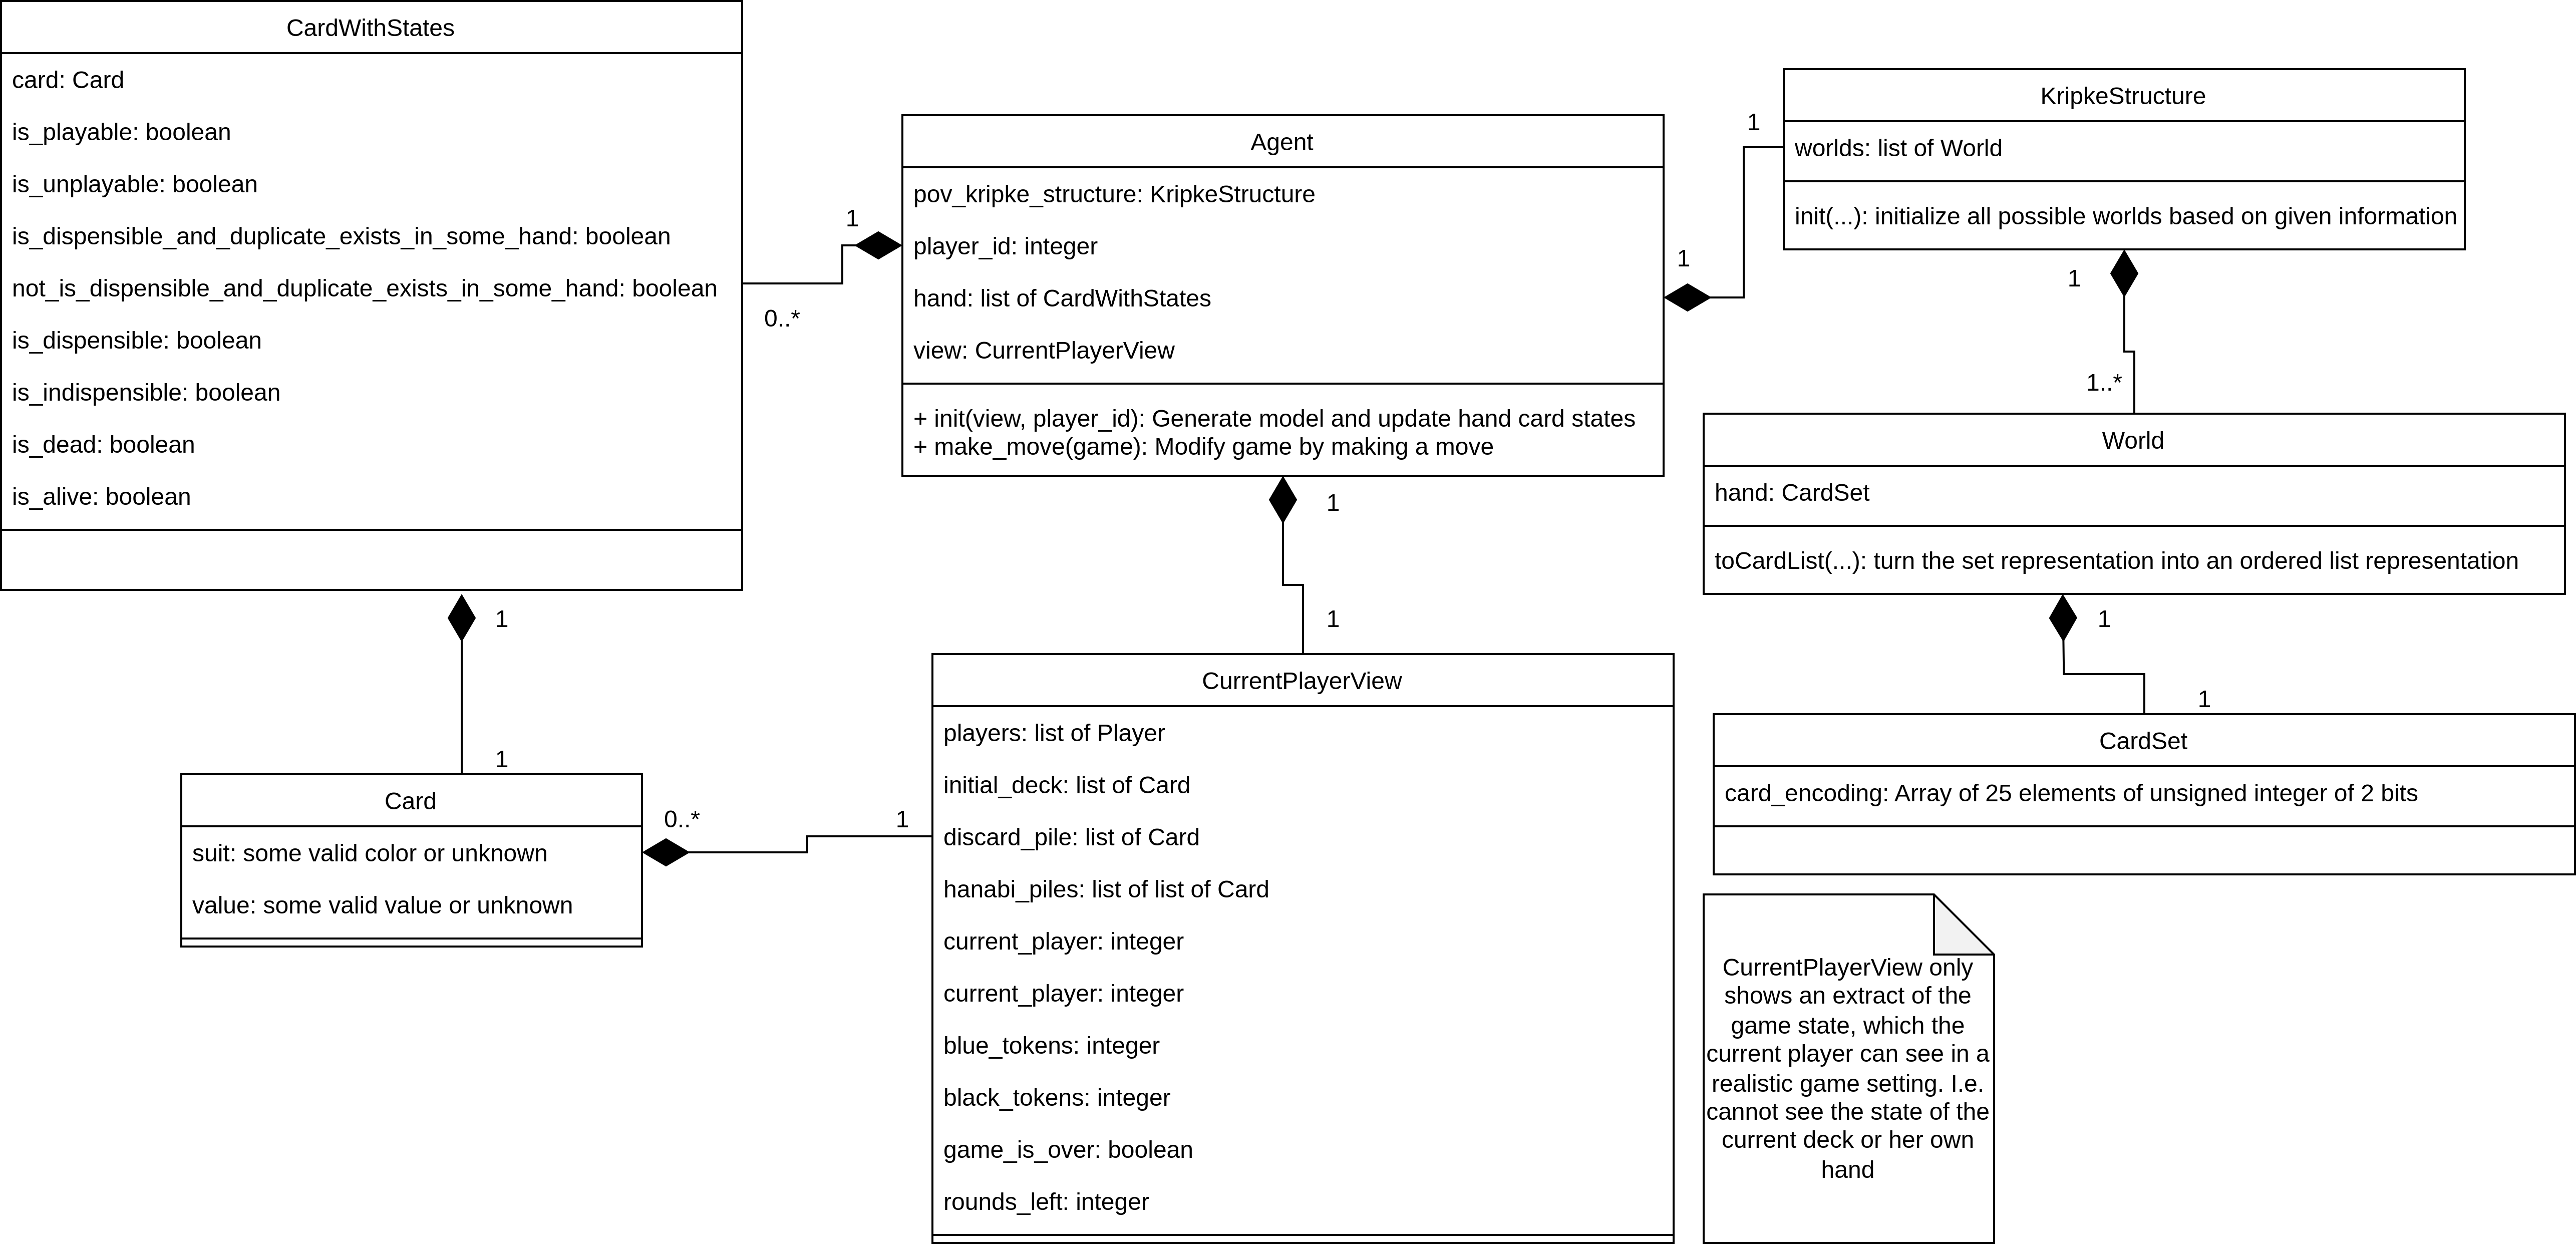
\includegraphics[width=23cm]{images/agent-uml-class-diagram.png}
	\caption{Low-fidelity class diagram for the things making up the Agent class}
	\label{fig:Agent-class-diagram}
\end{sidewaysfigure}

\subsection{Game simulation runner}
The glue-code between the Agents and the Game classes, is a class called SimulationRunner (defined in "{\tt src/ai\_simulation\_runner.zig}"), which takes a Game
